\documentclass[11pt]{article}
% The KINTORA case-study paper of the Parsimony project.  Status: SKELETON (2026-10-10).
% Plan: ../casestudies/kintora/PLAN.md.  Driver interface: ../casestudies/kintora/DRIVER-CONTRACT.md.
% Shares refs.bib with parsimony.tex; build both with `make`.  Prose follows
% ~/Codes/plasma-kinetics/paper/house-style.md ("mu row", never a bare "row"; "cell" is a
% triangle of the poloidal plane; every number has a source).  Sources of the KINTORA numbers
% are the ledger entries named in the comments (~/Codes/plasma-kinetics/plans/design-ledger.md).

\usepackage[margin=1in]{geometry}
\usepackage{amsmath,amssymb}
\usepackage{booktabs}
\usepackage{xcolor}
\usepackage{hyperref}
\usepackage[numbers,sort&compress]{natbib}
\usepackage{tikz}
\usetikzlibrary{positioning,fit,backgrounds}
\usepackage{tabularx}

\hypersetup{colorlinks=true,linkcolor=blue!50!black,citecolor=blue!50!black,
            urlcolor=blue!50!black}

% Draft scaffolding, as in paper/parsimony.tex: \pending is an argument the paper intends to
% make and has not yet earned; \todo is a smaller loose end.  Both render loudly on purpose.
\newcommand{\pending}[1]{%
  \par\medskip\noindent\fcolorbox{red!60!black}{red!4}{%
    \parbox{\dimexpr\linewidth-2\fboxsep-2\fboxrule}{\small\textbf{[PENDING]}\ #1}}%
  \par\medskip}
\newcommand{\todo}[1]{\textcolor{red!70!black}{\small[\textbf{TODO:} #1]}}
% The planning appendix (Appendix A): the design questions for Parsimony this study informs and
% the status of every section.  A design tool while the design is open; \planningfalse removes
% it, and the paper must still read complete without it.
\newif\ifplanning
\planningtrue
\newcommand{\plab}[1]{\ifplanning\ (P#1)\fi}
\newcommand{\vpar}{v_\parallel}
\newcommand{\code}[1]{\texttt{#1}}

\title{Precimonious and Blame Analysis Methods Applied to a\\
       Minimal-Precision Matrix-Free Multigrid Solve in a\\
       2X+1V Eulerian Solver for Magnetized Tokamak Plasmas}
\author{Mark F. Adams\\
        \small Lawrence Berkeley National Laboratory\\
        \small \texttt{mfadams@lbl.gov}}
\date{Draft --- \today}

\begin{document}
\maketitle

\begin{abstract}
The implicit stage of an Eulerian drift-kinetic solver for tokamak plasmas solves one linear
system per poloidal plane and magnetic moment, and on a GPU its cost is one V-cycle of a
matrix-free multigrid preconditioner per outer iteration.  Most of the bytes that V-cycle
holds are data it computes once and stores: per unknown, 24 values of block inverses for its
line smoother and 12 of face couplings.  Because these data only precondition an fp64
FGMRES iteration, their precision cannot move the converged answer; it changes the iteration
count.  This paper asks how few bits each stored quantity needs, and what those bits buy,
using the delta-debugging search of Precimonious and the attribution idea of Blame Analysis,
applied to the stored arrays of a GPU-resident solver rather than to the declared variables of
a serial program.  This paper builds on previous work on search-based precision tuning by
replacing error against an fp64 run with iterations at fixed residual tolerance and the
contraction factor of the V-cycle, and by making the multigrid level the unit of attribution.
\todo{the headline numbers, three or four, once Sections 5 and 6 are earned: the bits per
quantity at the knee, the v-resolution effect, the memory per GPU, the time per V-cycle.}
The study runs on NVIDIA A100 GPUs at NERSC, and it doubles as the second native-code
consumer of the Parsimony library, whose evaluator interface it settles.
\end{abstract}

% ---------------------------------------------------------------------------------------
\section{Introduction}
\label{sec:intro}

Implicit Eulerian schemes for drift-kinetic models of magnetized plasmas spend most of a time
step in linear solves.  KINTORA is a 3X+2V drift-kinetic code for tokamaks on unstructured,
flux-surface-aligned meshes~\cite{kintoramethods,kintorahpc}.  Its Eulerian solver advances the
ion distribution with an additive Runge--Kutta scheme~\cite{kennedycarpenter2003}, and each
implicit stage solves one linear system per poloidal plane and per $\mu$ row.  Each of these is a
2X+1V system in $(R, Z, \vpar)$, because the magnetic moment $\mu$ is an exact invariant and
nothing in the implicit operator couples two $\mu$ rows.  The solver is FGMRES on the fp64
operator, preconditioned by one V-cycle of a matrix-free geometric multigrid that runs on the
GPU.  On an NVIDIA A100 the V-cycle is the cost of the solve, and most of the bytes it holds are
data it computes once per $\mu$ row and stores: for each unknown, 24 values of the smoother's
block inverses and 12 of its face couplings (Section~\ref{sec:data}).

Those data only precondition.  FGMRES applies the fp64 operator and stops on its own residual,
so the precision of anything the V-cycle stores can change the number of iterations and not the
converged answer.  The precision of each stored quantity is therefore a free variable with a
measurable cost.  This paper asks how few bits each one needs.  One data point exists:
storing the block inverses in fp32 rather than fp64 left the outer iteration counts unchanged on
the three meshes tested, reduced the device arrays at the L5 mesh from 2.49\,GB to 1.91\,GB, and
cut the line-sweep kernel at L4 from 600\,$\mu$s to 490\,$\mu$s per call.
% D230(c)

Finding the fewest bits is a search problem, and the methods for it are a decade old.
Precimonious~\cite{precimonious} searches assignments of types to program variables with delta
debugging~\cite{ddmin} for one that meets an accuracy threshold and runs faster.  Blame
Analysis~\cite{blame} runs the program once under shadow execution, records for each instruction
the operand precision its result needs, and uses the record to prune Precimonious' search,
which it reports as $9\times$ faster on average and up to $38\times$.  Both were evaluated on
small serial programs against an error threshold relative to an fp64 run, as is the recent
PROMISE revival~\cite{promise2026}.  Our Parsimony paper~\cite{parsimony} reimplemented the
methods behind an interface that separates how a configuration is evaluated from how the space
is searched.  It found that for an iterative method the observable must be iterations at fixed
tolerance, and that the payoff of reduced precision depends on the storage format: on an A100,
fp32 storage made a blocked sparse matrix-vector product $1.75\times$ faster than fp64 and a
scalar seven-point stencil $1.07\times$ faster.

This paper applies both methods to KINTORA's V-cycle, which differs from the published
evaluations in three ways.  The variables are stored arrays of a GPU-resident solver, not
declared program variables, so rounding is applied where each array is written and the
arithmetic stays fp64.  The criterion is outer iterations at fixed residual tolerance, with a
continuous companion, the contraction factor of the V-cycle run as a stationary iteration,
because 2 to 4 outer iterations register only large changes in the preconditioner.  The solver
also has a stiffness parameter: at 48 $\vpar$ segments and large $\mu$, a smoother that resolves
only part of the $\vpar$ coupling stalls (Section~\ref{sec:cases}), and that is the regime where too
few bits are most likely to show.  Blame Analysis notes that for programs built on iterative
solvers, analyzing only the last few iterations is likely to suffice~\cite{blame}, so the choice
of what to analyze decides the cost.  Here the unit of attribution is a stored quantity on one
multigrid level.

The study is also a step in the design of the Parsimony library.  A lattice-QCD study of Grid's
multigrid preconditioner was the library's first consumer of a native GPU code, and its
evaluator was written for that code alone.  KINTORA is the second consumer.
Section~\ref{sec:workflow} reports what the two share and what moved into the library as a
result.

The contributions of this paper are:
\begin{itemize}
  \item An inventory of the stored data of a matrix-free GPU multigrid, ranked by bytes, and
    the rule that decides what may be rounded, including the observation that the finest
    level's operator is the outer operator and so is not a preconditioner variable
    (Sections~\ref{sec:data} and~\ref{sec:variables}).
  \item A storage-rounding harness whose fp32 setting reproduces the production fp32 path bit
    for bit, so that its iteration counts are the real ones for any format stored narrow and
    computed in fp64 (Section~\ref{sec:rounding}). \todo{earned at Stage A, gate 2}
  \item The bits each stored quantity needs on each level, at 12 and at 48 $\vpar$ segments,
    from a uniform floor, a blame-style per-quantity analysis and a grouped delta-debugging
    search (Section~\ref{sec:bits}). \todo{Stages B, C}
  \item The sensitivity of the V-cycle's contraction factor to the precision of the smoother's
    stored data, used as a measure of the smoother's margin across $\mu$, $\Delta t$ and $\vpar$
    resolution, and the changes to the solver it led to (Section~\ref{sec:bits}). \todo{Stage B}
  \item What those bits buy on an A100, in device memory and in time per V-cycle, with real
    reduced-precision storage, and a comparison of a searched per-quantity format with a
    per-block rule chosen by block conditioning (Section~\ref{sec:payoff}). \todo{Stage D}
  \item A workflow for applying search-based precision tuning to a native GPU solver, and the
    library interface it requires (Section~\ref{sec:workflow}).
\end{itemize}

% ---------------------------------------------------------------------------------------
\section{Background}
\label{sec:background}

\subsection{Precimonious}
Precimonious~\cite{precimonious} assigns each floating-point variable of an LLVM program a type
and searches the assignments with delta debugging~\cite{ddmin}, whose worst case is $O(n^2)$
evaluations in the number $n$ of variables.  A candidate passes if its output meets an error
threshold relative to the fp64 program and it runs faster.  Each evaluation recompiles and
reruns the program.  The search is empirical: a configuration found for one threshold does not
bound the configuration for another.

\subsection{Blame Analysis}
Blame Analysis~\cite{blame} replaces most of the search with attribution.  It executes each
floating-point instruction under shadow execution at several operand precisions at once, and
for a required precision of the result it records the smallest operand precisions that meet it.
A backward pass from the output yields the variables that may be lowered, and that set prunes
the Precimonious search.  The instruction-level analysis costs up to $50\times$ the program's
run time online, and offline its memory grows with the dynamic trace~\cite{blame}.

\subsection{Parsimony}
Parsimony~\cite{parsimony} reimplements both methods behind two protocols: an \emph{evaluator},
which scores one precision configuration, and a \emph{search}, which proposes configurations
(a uniform bisection, a solo-sensitivity prefilter in the role of Blame Analysis, and delta
debugging).  Its formats are the IEEE and vendor formats (fp32, tf32, bf16, fp16, two fp8
encodings) and \emph{virtual} formats $v_k$, a float64 rounded to $k$ significand bits, which
ask how many bits a value needs without committing to a storage layout.  What its evaluators
model is \emph{storage}: each named value is rounded where it is produced and the arithmetic
stays fp64.  Three of its findings shape this study.  For an iterative method, error against
an fp64 run measures the reproduction of a rounding trajectory, not solution quality, so the
criterion is iterations at fixed residual tolerance (\code{IterationBudget}).  Floors found one
variable at a time are not sound bounds, because a coarse format downstream can absorb error
from upstream.  A single input lets the search quantize its output onto a lucky lattice point,
so every evaluation uses several cases.

\subsection{The structure of the Parsimony project}
\label{sec:shape}
Figure~\ref{fig:shape} shows the parts of the project and where this study enters.  The core
is a Python package that knows nothing about any application: the formats and their emulation,
the criteria that decide whether a configuration passes, and the searches.  It is tested against
synthetic oracles, so a search can be checked independently of any floating-point emulation.
An application enters only through an \emph{evaluator}, which takes a configuration and returns
a scored result.  The built-in evaluator runs Python kernels whose named values are rounded on
the fly; the Parsimony paper's conjugate-gradient and Newton studies use it.  A compiled code
needs more: a rounding header compiled into the application at its storage points, a
contract for how a configuration reaches the application and how the result comes back, and an
evaluator that manages the application's processes.  The Grid study built these three for Grid
alone.  This study is the second consumer of that native layer, and the parts the two studies
share are the ones that move into the library (Section~\ref{sec:workflow}).  The sparse
matrix-vector and PETSc end-to-end studies of the Parsimony paper measured cost per iteration
with real reduced-precision builds and used no evaluator; a timed evaluator would bring that
measurement inside the search.

\begin{figure}[tbp]
  \centering
  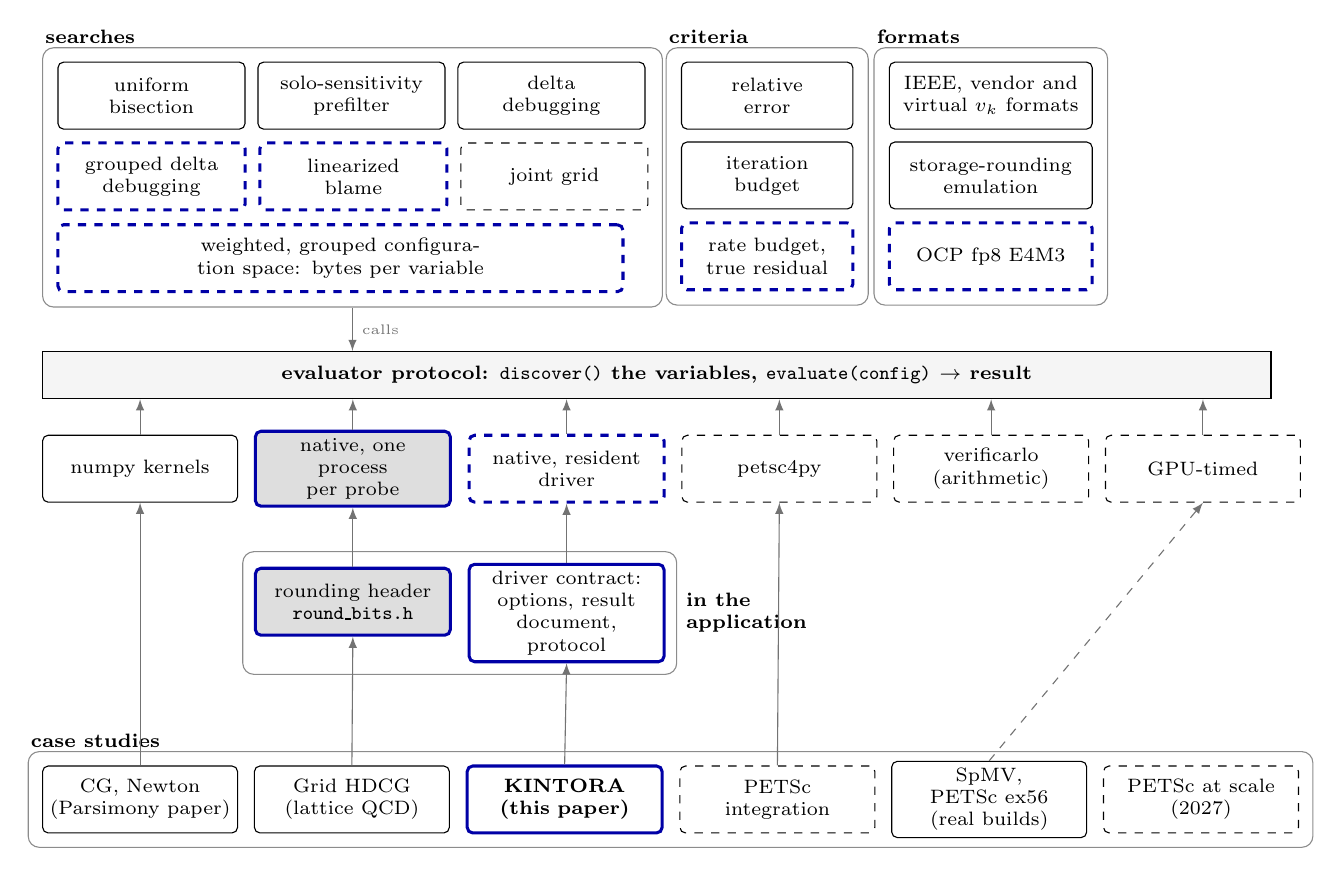
\begin{tikzpicture}[
      font=\scriptsize,
      b/.style={draw, rounded corners=2pt, align=center, inner sep=2.5pt,
                minimum height=0.85cm, text width=#1},
      b/.default=2.2cm,
      improv/.style={fill=black!13},
      planned/.style={dashed},
      ours/.style={draw=blue!65!black, line width=1.1pt},
      grp/.style={draw=black!45, rounded corners=4pt, inner sep=5pt},
      glab/.style={font=\scriptsize\bfseries, anchor=south west, inner sep=1pt},
      arr/.style={-latex, black!55}]
    % ---- the core
    \node[b] (uni) at (0,0) {uniform\\bisection};
    \node[b, right=0.15cm of uni] (solo) {solo-sensitivity\\prefilter};
    \node[b, right=0.15cm of solo] (dd) {delta\\debugging};
    \node[b, planned, ours, below=0.15cm of uni] (grp) {grouped delta\\debugging\plab{6}};
    \node[b, planned, ours, right=0.15cm of grp] (lin) {linearized\\blame\plab{7}};
    \node[b, planned, right=0.15cm of lin] (joint) {joint grid\plab{8}};
    \node[b=2.0cm, right=0.45cm of dd] (rel) {relative\\error};
    \node[b=2.0cm, below=0.15cm of rel] (itb) {iteration\\budget};
    \node[b=2.0cm, planned, ours, below=0.15cm of itb] (rate) {rate budget,\\true residual\plab{4}};
    \node[b=2.4cm, right=0.45cm of rel] (fmt) {IEEE, vendor and\\virtual $v_k$ formats};
    \node[b=2.4cm, below=0.15cm of fmt] (emu) {storage-rounding\\emulation};
    \node[b=2.4cm, planned, ours, below=0.15cm of emu] (e4m3) {OCP fp8 E4M3\plab{0}};
    \node[b=7.0cm, planned, ours, below=0.15cm of grp.south west, anchor=north west]
         (space) {weighted, grouped configuration space: bytes per variable\plab{5}};
    \begin{scope}[on background layer]
      \node[grp, fit=(uni)(joint)(space)] (gS) {};
      \node[grp, fit=(rel)(rate)] (gC) {};
      \node[grp, fit=(fmt)(e4m3)] (gF) {};
    \end{scope}
    \node[glab] at (gS.north west) {searches};
    \node[glab] at (gC.north west) {criteria};
    \node[glab] at (gF.north west) {formats};
    % ---- the evaluator protocol
    \node[draw, fill=black!4, minimum height=0.6cm, minimum width=15.6cm, anchor=north west,
          font=\scriptsize\bfseries] (proto) at ([yshift=-0.55cm]gS.south west)
          {evaluator protocol: \texttt{discover()} the variables, \texttt{evaluate(config)} $\to$ result};
    % ---- evaluators
    \node[b=2.3cm, anchor=north west] (np) at ([yshift=-0.45cm]proto.south west) {numpy kernels};
    \node[b=2.3cm, improv, ours, right=0.2cm of np] (nat) {native, one process\\per probe\plab{2}};
    \node[b=2.3cm, planned, ours, right=0.2cm of nat] (res) {native, resident\\driver\plab{3}};
    \node[b=2.3cm, planned, right=0.2cm of res] (p4p) {petsc4py};
    \node[b=2.3cm, planned, right=0.2cm of p4p] (vfc) {verificarlo\\(arithmetic)};
    \node[b=2.3cm, planned, right=0.2cm of vfc] (tim) {GPU-timed};
    % ---- inside the application
    \node[b=2.3cm, improv, ours, anchor=north] (hdr) at ([yshift=-0.75cm]nat.south)
         {rounding header\\\texttt{round\_bits.h}\plab{1}};
    \node[b=2.3cm, ours, anchor=north] (con) at ([yshift=-0.75cm]res.south)
         {driver contract:\\options, result\\document, protocol};
    \begin{scope}[on background layer]
      \node[grp, fit=(hdr)(con), inner sep=4pt] (gA) {};
    \end{scope}
    \node[glab, anchor=west, align=left] at ([xshift=2pt]gA.east) {in the\\application};
    % ---- case studies
    \node[b=2.3cm, anchor=north west] (cg) at ([yshift=-1.15cm]np.south west |- gA.south) {CG, Newton\\(Parsimony paper)};
    \node[b=2.3cm, right=0.2cm of cg] (grid) {Grid HDCG\\(lattice QCD)};
    \node[b=2.3cm, ours, right=0.2cm of grid] (kin) {\textbf{KINTORA}\\\textbf{(this paper)}};
    \node[b=2.3cm, planned, right=0.2cm of kin] (petsc) {PETSc\\integration};
    \node[b=2.3cm, right=0.2cm of petsc] (spmv) {SpMV, PETSc ex56\\(real builds)};
    \node[b=2.3cm, planned, right=0.2cm of spmv] (scale) {PETSc at scale\\(2027)};
    \begin{scope}[on background layer]
      \node[grp, fit=(cg)(scale)] (gK) {};
    \end{scope}
    \node[glab] at (gK.north west) {case studies};
    % ---- edges
    \draw[arr] (gS.south) -- (gS.south |- proto.north) node[midway, right, font=\tiny] {calls};
    \draw[arr] (np.north) -- (np.north |- proto.south);
    \draw[arr] (nat.north) -- (nat.north |- proto.south);
    \draw[arr] (res.north) -- (res.north |- proto.south);
    \draw[arr] (p4p.north) -- (p4p.north |- proto.south);
    \draw[arr] (vfc.north) -- (vfc.north |- proto.south);
    \draw[arr] (tim.north) -- (tim.north |- proto.south);
    \draw[arr] (cg.north) -- (np.south);
    \draw[arr] (grid.north) -- (hdr.south);
    \draw[arr] (kin.north) -- (con.south);
    \draw[arr] (petsc.north) -- (p4p.south);
    \draw[arr, dashed] (spmv.north) -- (tim.south);
    \draw[arr] (hdr.north) -- (nat.south);
    \draw[arr] (con.north) -- (res.south);
  \end{tikzpicture}
  \caption{The parts of the Parsimony project.  Solid boxes exist in the library, grey boxes
    exist inside one case study only (the Grid study's evaluator and rounding header), dashed
    boxes are planned, and blue outlines mark what this study needs or adds\ifplanning; the labels P0 to P8
    are the items of Appendix~\ref{app:plan}\fi.  The core (top) does not depend on any
    application; an application enters only through an evaluator, and a compiled application
    through the native layer below the evaluator protocol.  The SpMV and ex56 studies measured
    cost with real reduced-precision builds outside any evaluator (dashed arrow).}
  \label{fig:shape}
\end{figure}

% ---------------------------------------------------------------------------------------
\section{The solver and the data it stores}
\label{sec:solver}

\subsection{The implicit stage}
The unknown is the ion distribution $f(R, Z, \vpar, \mu)$ on one poloidal plane.  The implicit
operator contains the parallel streaming, the mirror force, the magnetic drift and the drift's
energy exchange; every term that reads the electrostatic potential is explicit.  An implicit
stage of the scheme, with stage weight $\gamma = 0.4359$ and time step $\Delta t$, solves
\begin{equation}
  K f = \left( \frac{M_J}{\gamma\,\Delta t} + A_s + \mu A_m \right) f = r
  \label{eq:stage}
\end{equation}
for each $\mu$ row, with $M_J$ the mass matrix weighted by the guiding-centre Jacobian and $A_s$,
$A_m$ the transport operators of a discontinuous Galerkin (DG) discretization with upwind
fluxes.  Each cell (a triangle of the flux-aligned poloidal mesh) carries a $P_2$ space in the
plane and a $P_3$ space on each of 12 $\vpar$ segments, nodal at four Gauss--Lobatto points, so
a $\mu$ row has 288 unknowns per cell.  The meshes form a series L0 to L6 of $16 \cdot 4^L$
cells; a $\mu$ row has $1.18 \times 10^6$ unknowns at L4, $4.72 \times 10^6$ at L5 and
$1.89 \times 10^7$ at L6, and the velocity grid has 24 $\mu$ rows.  KINTORA's model is 3X+2V;
the solver measured here is its axisymmetric configuration, in which the implicit operator has
no toroidal coupling and each solve is the 2X+1V system above.
% gamma: ARKIMEX3 (kin_gate_eul.cxx: 1767732205903/4055673282236).  Sizes: 288 = 12 x 4 x 6.

The fp64 operator conserves mass, energy and the canonical toroidal momentum to round-off,
because the discrete flux field is orthogonal to the gradients of the discrete Hamiltonian and
of the flux function at every quadrature point; on the A100 we measured conservation defects of
at most $7 \times 10^{-16}$ per step over 500 steps.  This property belongs to $K$, not to the
preconditioner, and it is one reason the outer operator stays fp64.
% D222 (the identities), D230(d) (ledgers <= 7e-16 per step).
\todo{cite the Eulerian solver paper once it exists.}

\subsection{The preconditioner}
\label{sec:pc}
FGMRES (restart 30, relative tolerance $10^{-10}$) solves $J f = b$ with $J = M_J^{-1} K$, right
preconditioned by one V-cycle on $K$ applied to $M_J b$.  The multigrid levels rediscretize
Equation~(\ref{eq:stage}) on the coarser meshes of the series, which are not nested; the transfer
between levels is one $6 \times 6$ block per fine cell, and $\vpar$ is never coarsened.  Every
level above L0 is matrix-free: its operator applies $K$ from tables of the geometry at the
quadrature points.  L0 is assembled and solved by NVIDIA's cuDSS direct solver.  The smoother is
three Richardson steps before and after the coarse correction, V(3,3), each preconditioned by a
line sweep: the cells of each flux-surface ring are cut into arcs (64 cells on the finest level,
halved on each coarser level), and along each arc a forward and a backward sweep solve with the
$24 \times 24$ block of one cell and $\vpar$ segment exactly and with the face coupling to the
neighbouring cell of the arc.  Upwinding makes the coupling along an arc one-sided in walk
order wherever the streaming along it is one-signed, and there the two sweeps solve the line
exactly: with V(2,2) and arcs of 16 cells we measured the same outer iteration counts as with
sparse LU factors of the lines, case for case.  The coupling between adjacent $\vpar$ segments
is not in the line solve.
% D229(b), D230(c): "the 24 x 24 sweep at V(2,2) arcs 16 has EXACTLY the LU lines' outer counts".

On one A100 the solve at L4, summed over nine cases ($\mu$ rows 0, 12 and 23 at
$\Delta t = 0.05$, 0.2 and 0.4), takes 0.65\,s of set-up and solve with 2 or 3 outer iterations
per case; at L5 it takes about 2.0\,s with 2 to 4.  At L6 ($1.89 \times 10^7$ unknowns per
$\mu$ row, seven levels), with arcs of 128 cells on the finest level, a stage solve on $\mu$ rows 12
and 23 at $\Delta t = 0.2$ and 0.4 takes 0.51 to 0.69\,s in 3 to 5 iterations, and the run holds
10.5\,GB of device memory.
% D230(c); L6: arcs 128 + fp32 (session-8 brief item 0, ~/eul/L6b_node.txt).

\subsection{The stored data}
\label{sec:data}
Table~\ref{tab:data} lists what the V-cycle stores, by values per unknown of one $\mu$ row.  Two
arrays dominate.  The block inverses hold 24 values per unknown and the face couplings 12;
both are recomputed for each $\mu$ row and $\Delta t$, and both are read on every application of
the smoother.  Summed over the matrix-free levels L1 to L5, the block inverses at fp64 hold
$6.29 \times 10^6 \times 24 \times 8\,\mathrm{B} = 1.21$\,GB, so storing them in fp32 should save
0.60\,GB; the measured reduction is 0.58\,GB (2.49 to 1.91\,GB).  With the inverses in fp32,
the face couplings at fp64 (0.60\,GB at L5) are as large as the inverses.  The operator tables
and the transfer blocks are smaller by an order of magnitude or more, so their precision can
matter to the convergence and not to the memory or the traffic.
\todo{units of KINTORA's memory report (GB or GiB) and the triangle rule's point count, from
\code{-kin\_mem\_view} and the \code{eulgeom} view line.}

\begin{table}[tbp]
  \centering
  \footnotesize
  \caption{The arrays a V-cycle of one $\mu$ row stores on the device, in values per unknown of
    the level, from the allocation sizes in KINTORA's \code{kin\_eulop.kokkos.cxx} (commit
    \code{7f8c9d9}).  ``Rounded'' says whether the array is a variable of this study
    (Section~\ref{sec:variables}).}
  \label{tab:data}
  \begin{tabular}{@{}llrlll@{}}
    \toprule
    quantity & array & per unknown & computed & read by & rounded \\
    \midrule
    block inverses $D^{-1}$ ($24 \times 24$) & \code{d\_sw24} & 24 & each $\mu$ row, $\Delta t$ & sweep & every level \\
    face couplings $C$ ($6 \times 6$) & \code{d\_sweepg} & 12 & each $\mu$ row, $\Delta t$ & sweep & every level \\
    V-cycle vectors & \code{Vec} & about 6 & each V-cycle & all kernels & every level \\
    operator tables & \code{d\_mf} & 2.3--2.6 & once & operator & below the finest \\
    transfer blocks & \code{d\_pblk} & 0.125 & once & transfers & every level \\
    node blocks & \code{d\_pbinv} & 6 & each $\mu$ row, $\Delta t$ & set-up only & no \\
    $M_J^{-1}$ blocks & \code{d\_Minv} & 6 & once & outer operator & no \\
    \bottomrule
  \end{tabular}
\end{table}

% ---------------------------------------------------------------------------------------
\section{Method}
\label{sec:method}

\subsection{Variables, and what may be rounded}
\label{sec:variables}
Only preconditioner input is rounded.  The outer operator $J$ and FGMRES stay fp64, so the
converged answer and the conservation of the step do not depend on the configuration.  The
finest level of the V-cycle needs care here, because it is the outer operator: the multigrid's
finest-level operator object and FGMRES's $J$ apply the same matrix-free $K$ from the same
tables.  Rounding the finest level's operator tables would change the matrix FGMRES converges
on.  The operator tables are therefore rounded on the levels below the finest only; the finest
level's would need a second, rounded copy, which production would also have to store.  The
block inverses, the face couplings, the transfer blocks and the vectors are preconditioner-only
on every level.

The variables are six quantities on each matrix-free level: \code{dinv} ($D^{-1}$),
\code{coup} ($C$), \code{kmf} (the operator tables), \code{prol} (the transfer blocks),
\code{vx} (the smoother's iterate and the prolonged correction) and \code{vr} (the residual and
the restricted right-hand side).  The vectors are two variables, not one, because a stored
residual and a stored iterate behave differently: in the Parsimony study of Newton's method the
residual could be stored in 16 bits but not evaluated in fewer than 33~\cite{parsimony}.  A level
is named by its depth below the finest, so a configuration found at L4 applies at L5.  At L4,
with four matrix-free levels and no finest-level operator tables, the space has 23 variables.

\subsection{Storage rounding and its checks}
\label{sec:rounding}
Each variable is rounded at the point its array is written, by a header shared with the
Parsimony library that rounds a double to nearest, ties to even, in any of the formats of
Section~\ref{sec:background}, and agrees bit for bit with the library's emulation.  One
command-line option per variable sets its format on each level, and an unknown format stops the
run.  Three checks qualify the harness before any result is read from it.
\begin{itemize}
  \item With every variable at $v_{53}$, the outer iteration counts and residual histories equal
    those of the unmodified code bit for bit.
  \item Rounding $D^{-1}$ to fp32 reproduces KINTORA's production fp32 path bit for bit.  That
    path casts each inverse entry to \code{float} when it is stored and converts it back to
    fp64 when the sweep reads it, which is storage rounding with fp64 arithmetic.  The match
    shows the hook acts on the value the sweep consumes, and it means that the iteration counts
    this harness reports are the real ones for any format implemented the same way.
  \item Every rounded array reports the relative change the rounding made, and a zero where a
    change was requested stops the search, because a hook attached to the wrong object produces a
    flat curve that cannot be told from a free variable.
\end{itemize}
\pending{Stage A: the three checks run and pass on L2 (Mac) and L4 (A100).}

\subsection{Observables and criteria}
\label{sec:observables}
The primary observable is the number of outer FGMRES iterations to the relative tolerance
$10^{-10}$, judged by Parsimony's \code{IterationBudget}: a configuration passes if every case
converges within $\lceil (1 + s)\, n_\mathrm{ref} \rceil$ iterations, with $s$ the slack and
$n_\mathrm{ref}$ the fp64 count.  Each solve also reports an independent true residual
$\|b - J f\|_2 / \|b\|_2$ computed with the unrounded $J$, so that a configuration under which
the solver stops on a residual it computed wrongly fails.  At 2 to 4 iterations a count
changes only when the preconditioner degrades by 25\% to 50\%, so the second observable is the
contraction factor $\rho$ of the V-cycle run as a stationary iteration,
$f \leftarrow f + \mathrm{MG}(M_J (b - J f))$: the geometric mean of the residual reduction per
cycle over 20 cycles or down to $10^{-12}$, which KINTORA's solve test already reports.  The
criterion \code{RateBudget} passes a configuration whose $\rho$ stays within a factor $1 + s$ of
the fp64 value in every case.  The contraction factor resolves degradation that does not yet
cost an outer iteration, and it is the observable the blame-style analysis of
Section~\ref{sec:searches} needs.
\todo{the noise floor of $\rho$: the spread over repeated fp64 runs, which bounds the smallest
resolvable degradation.}

\subsection{Cases}
\label{sec:cases}
The base set is nine cases, $\mu$ rows 0, 12 and 23 at $\Delta t = 0.05$, 0.2 and 0.4, at 12
$\vpar$ segments: three $\mu$ rows and three time steps, because the iteration count is
quantized and one case can be lucky.  The stiff set is four cases at 48 $\vpar$ segments,
$\mu$ rows 18 and 23 at $\Delta t = 0.2$ and 0.4.  A sweep whose diagonal block is one $\vpar$
node's $6 \times 6$ block, which leaves the coupling between the four nodes of a segment to the
Richardson iteration, converges at L2 in at most 10 iterations at 12 segments.  At 48 segments
the same sweep did not converge in 200 iterations on $\mu$ rows 18 and 23 at $\Delta t = 0.2$, and
in a time-dependent run at L4 it left FGMRES flat at a relative residual of $3 \times 10^{-5}$ on
$\mu$ row 18.  The sweep with the $24 \times 24$ block of the whole segment converges in 2 to 4
iterations on the same cases.
% D230(b): Mac L2 v48 rows 18/23 dt .2: 6x6 sweep 200 (DIVERGED_ITS), 24x24 sweep 2; L2 v12 all
% <= 2 except row 23 dt .4 (10); P1.3 L4 v48 row 18 flat at 3e-5.  D230(c): L4 v48 rows 18/23 2-4 its.
The coupling between adjacent $\vpar$ segments is still left to the Richardson iteration, so the
stiff set is where the smoother has the least margin.

\subsection{Searches}
\label{sec:searches}
Four searches run in order of cost, each on the outputs the previous one cached.
\begin{enumerate}
  \item \textbf{Uniform floor}: every variable at one format, bisected over the format ladder.
    This is the configuration a code would choose with one global setting, and the baseline
    against which the mixed configuration is worth its search.
  \item \textbf{Blame-style attribution}: each variable alone at a fine virtual width, the
    others at fp64.  The change in $\rho$ gives a sensitivity coefficient $c_v$ per variable.
    If the degradation is linear in the rounding error, which scales as $2^{-k}$ at $k$ bits,
    the knee of variable $v$ is at $k_v = \log_2 (c_v / \delta)$ for a tolerated degradation
    $\delta$, and the cheapest joint configuration under the same model spends bits where the
    marginal degradation per byte is equal.  This is Blame Analysis' idea at the granularity of
    stored quantities: one inexpensive pass per variable predicts the configuration, and the
    search confirms or refutes the prediction.
  \item \textbf{Grouped delta debugging}: Parsimony's delta debugging over the six quantities
    with all levels of a quantity together, then over the levels inside each quantity that was
    lowered, in the manner of hierarchical delta debugging~\cite{hdd}.  The objective counts
    bytes, weighting each variable by the values it stores per unknown
    (Table~\ref{tab:data}); unweighted, the search would report a lowered transfer block as a
    gain.
  \item \textbf{Joint grid} over $D^{-1}$ and $C$, the two largest arrays, at every pair of
    formats on the ladder.  One-at-a-time floors are not sound bounds when errors
    interact~\cite{parsimony}, and the two arrays enter the same sweep step.
\end{enumerate}
The ladder for the search is virtual widths $v_{53}$, $v_{40}$, $v_{30}$, $v_{24}$, $v_{16}$,
$v_{11}$ and $v_8$.  The named formats (fp32, tf32, fp16, bf16, fp8) are evaluated afterwards
at the knees, because a result that is to be deployed has to name a format that hardware
stores.  The fp8 E4M3 format follows the OCP definition~\cite{ocpfp8}, with a largest
finite value of 448 and no infinity, as hardware implements it; an overflow is NaN.

\subsection{The evaluator}
\label{sec:evaluator}
A probe is one configuration evaluated on every case.  The driver is KINTORA's test executable,
kept resident: it builds the meshes, the geometry tables and the hierarchy once, then reads one
configuration per line, restores every rounded set-up array from a pristine fp64 copy, applies
the formats, runs the cases and writes one result document per line.  At L4 the set-up of a
process takes about a minute against 0.65\,s for the set-up and solve of the nine cases, so a
resident driver turns hours of search into minutes.  The result document carries the
configuration as applied, the relative change each rounding made, and per case the convergence
reason, the iteration count, the true residual, $\rho$ and the times; it also records the
KINTORA commit and the full option string, because a precision result is a property of the
algorithm (the arc length, the cycle, the block size, the segment count) and must be rerun when
any of them changes.  The base and stiff sets use different $\vpar$ grids and therefore two
resident drivers, which one evaluator queries together.
\todo{the one-minute set-up figure is the PLAN's estimate; measure it at L4.}

% ---------------------------------------------------------------------------------------
\section{How many bits}
\label{sec:bits}

\pending{\textbf{Uniform floor} (Stage B at L2, Stage C at L4): the lowest single format for every
variable at slack 0 and 0.25, on the base set and on the stiff set separately.  Prediction to test:
the stiff set's floor is higher.}

\pending{\textbf{Per-quantity knees} (Stage B, C): for each quantity, $\rho$ and the outer iterations
against bits, all levels together; a table of $k_v$ predicted by the blame-style coefficients
against $k_v$ found by bisection.  Also the condition numbers of the $24 \times 24$ blocks per
$\mu$ row and $\Delta t$, the predictor of Anzt et al.~\cite{anzt2019adaptive}.}

\pending{\textbf{The mixed configuration} (Stage C): the grouped search's result at L4 at slack 0 and
0.25, its bytes against the uniform floor's, its probe count against ungrouped delta debugging,
and whether the joint grid over $D^{-1} \times C$ finds a configuration the one-at-a-time search
missed.}

\pending{\textbf{What the bits say about the smoother} (Stage B): rounding $D^{-1}$ is a
controlled perturbation of the smoother, so the rate at which $\rho$ degrades as bits are removed
measures how much margin the smoother has.  The map of that rate over $\mu$, $\Delta t$ and the
$\vpar$ resolution locates where the smoother is closest to failing, which is the regime of
Section~\ref{sec:cases} where the coupling between $\vpar$ segments is left to the Richardson
iteration.  Prediction to test: the sensitivity grows with $\mu$ and with the number of segments,
and it is largest where a smoother that omits the inter-segment coupling would need it.  Report
what KINTORA changed as a result, if anything.}

\pending{\textbf{Levels and resolution} (Stage C): whether a level's requirement follows its depth
below the finest or its mesh (the in-plane streaming Courant number is 7, 16 and 32 on L2, L3 and
L4 at $\Delta t = 0.2$); 12 against 48 $\vpar$ segments; the L4 configuration confirmed at L5 and
L6.}

% ---------------------------------------------------------------------------------------
\section{What the bits buy}
\label{sec:payoff}

Reduced storage buys memory unconditionally and time only where a kernel is
bandwidth-bound.  The line sweep is not: with fp32 inverses at L4 it runs 780 lines of 24
lanes, 195 thread teams, at 8\% occupancy, latency-bound with too few warps resident to hide the
latency of its sequential chain along the arc.  Halving the bytes of its inverses made it
$1.22\times$ faster (600 to 490\,$\mu$s).  The time the remaining bits can buy therefore depends
on the sweep's parallelism, which is under development, and Section~\ref{sec:bits}'s answers do
not: they depend on what the V-cycle computes, not on how the kernel schedules it.
% D230(c): "ncu: 195 teams, 8% occupancy, latency-bound: 780 lines x 24 lanes"

\pending{\textbf{Memory} (Stage D): device memory per array at L5 and L6 with real storage at the
knee formats (\code{-kin\_mem\_view}), and the finest mesh one 40\,GB A100 holds.  The L6 run holds
10.5\,GB with fp32 inverses; the arithmetic of Table~\ref{tab:data} gives the inverses and couplings
4.83\,GB and 2.42\,GB at fp64 over L1 to L6.}

\pending{\textbf{Time} (Stage D, after the sweep's parallelism work): time per V-cycle and per stage
solve with real 16-bit storage of $D^{-1}$ and $C$, against emulated iteration counts; the check that
the two counts agree.}

\pending{\textbf{A rule against a search} (Stage D): per-block storage formats chosen from each block's
condition number~\cite{anzt2019adaptive,flegar2021ginkgo}, against the searched per-quantity format,
in bytes and iterations.}

% ---------------------------------------------------------------------------------------
\section{The workflow and the structure of Parsimony}
\label{sec:workflow}

Applying the methods to a native GPU solver took eight steps, and each one either used a piece of
the Parsimony library or exposed a missing one.
\begin{enumerate}
  \item \textbf{Inventory} the stored data by bytes per unknown and by who reads it
    (Table~\ref{tab:data}).  The inventory supplies the search's variables and their weights.
  \item \textbf{Classify} each array as preconditioner input, operator, or shared between the
    two.  Only the first may be rounded without a second copy.
  \item \textbf{Hook} the store sites with the library's rounding header, one option per variable,
    with unknown formats rejected.
  \item \textbf{Verify} the hooks positively (Section~\ref{sec:rounding}).
  \item \textbf{Choose} observables that resolve the effect and cases that include the stiff regime
    (Sections~\ref{sec:observables} and~\ref{sec:cases}).
  \item \textbf{Search} in order of cost: uniform, attribution, grouped delta debugging, joint grid
    (Section~\ref{sec:searches}).
  \item \textbf{Realize} the knee formats in real storage and measure memory and time
    (Section~\ref{sec:payoff}).
  \item \textbf{Tabulate} every number in the paper from the result documents by script.
\end{enumerate}

The Grid study improvised steps 3, 4 and 6 for one code: a rounding header, an evaluator that
runs the driver once per configuration, caches every result and refuses a run that wrote no
result, and a check that every requested rounding changed something.  KINTORA needs the same
pieces and adds four the library lacked: a resident driver with a line protocol (step 6's cost),
a contraction-factor criterion (step 5), weights on the variables (step 1) and grouped variables
with a group-then-refine search (step 6).  The second consumer is the point at which the common
part can be identified.  The interface it settles is a document schema and a line protocol that
any driver can implement in its own language, so the library never links against the solver
and the solver never depends on the library.
\pending{what moved into \code{src/parsimony/} and the tests that hold each piece (PLAN.md, track
P), and the Grid evaluator rerun on the extracted base with unchanged results.}

% ---------------------------------------------------------------------------------------
\section{Limitations}
\label{sec:limitations}

\paragraph{Storage, not arithmetic.}  The harness rounds what is stored and computes in fp64.  For
formats implemented the same way the counts are exact (Section~\ref{sec:rounding}); for an
implementation that also computes in reduced precision, such as the set-up's $24 \times 24$
Gauss--Jordan inversion in fp32, they are optimistic.  An arithmetic evaluator, verificarlo's
variable-precision backend~\cite{verificarlo}, runs on KINTORA's CPU build only, because it
instruments LLVM code and cannot see CUDA kernels; it would test the set-up's arithmetic at L2.

\paragraph{One GPU.}  Every measurement is on one A100.  The solve is per $\mu$ row and the
$\mu$ rows are distributed over GPUs without communication inside a solve, so the per-GPU result
carries over to more GPUs at a fixed number of $\mu$ rows per GPU; a plane decomposition inside
a $\mu$ row would add halo traffic that this study does not measure.

\paragraph{The axisymmetric solve.}  The study measures the 2X+1V solve of the axisymmetric code.
A three-dimensional implicit operator, with streaming along the toroidal angle between wedges,
would change the smoother and require the study to be repeated.

\paragraph{One equilibrium and one profile set.}  The cases are one Solov'ev equilibrium with one
set of density and temperature profiles.  The stiffness knobs the study varies are the $\vpar$
resolution, $\mu$ and $\Delta t$.

% ---------------------------------------------------------------------------------------
\section{Related work}
\label{sec:related}

\paragraph{Precision tuning.}  Precimonious~\cite{precimonious} and Blame
Analysis~\cite{blame} are the direct ancestors; HiFPTuner~\cite{hifptuner} groups variables by
the program's dependence structure before searching, which is the same move as this paper's
grouping by stored quantity.  PROMISE with customized precisions~\cite{promise2026} revives the
search from the CADNA lineage on serial benchmarks.  Verificarlo~\cite{verificarlo} and
Verrou~\cite{verrou} change the arithmetic's rounding by compiler and binary instrumentation.

\paragraph{Reduced precision in multigrid and block preconditioners.}  Göddeke et
al.~\cite{goeddeke2007} ran multigrid in single precision inside a double-precision outer
iteration on early GPUs, and Kronbichler and Ljungkvist~\cite{kronbichler2019} run a matrix-free
high-order multigrid V-cycle in single precision as the preconditioner of a double-precision
conjugate gradient.  McCormick, Benzaken and Tamstorf~\cite{mccormick2021,tamstorf2021} analyze
how the precision of each multigrid component limits the attainable accuracy.  Closest to the
question of this paper, Anzt et al.~\cite{anzt2019adaptive,flegar2021ginkgo} store each
diagonal block inverse of a block-Jacobi preconditioner in fp64, fp32 or fp16 chosen from that
block's condition number.  This paper's $D^{-1}$ is such a set of block inverses inside a line
smoother, and Section~\ref{sec:payoff} compares their rule with a search.
\todo{check each characterization in this paragraph against the paper it cites; the entries are
[unverified] in refs.bib.}

\paragraph{The solver.}  The multigrid descends from the defect-correction construction of
Adams, Samtaney and Brandt~\cite{AdamsSamtaneyBrandt2010}, here as FGMRES on the high-order
operator with one V-cycle as the preconditioner.  It is built on PETSc~\cite{petsc} and
Kokkos~\cite{kokkos}.

% ---------------------------------------------------------------------------------------
\section{Conclusion}
\label{sec:conclusion}

\pending{The three or four numbers that matter (bits per quantity at the knee, the stiff set's
effect, memory per GPU, time per V-cycle), what the methods cost in probes on a production solver,
and the deferred work ranked: arithmetic precision of the set-up, the per-block rule at scale, and
the three-dimensional implicit operator.}

% ---------------------------------------------------------------------------------------
\section*{Code and Data Availability}

Parsimony, the evaluator and the result documents behind every table are at
\url{https://github.com/markadams/parsimony} (\code{casestudies/kintora/}).  KINTORA is at
\todo{the KINTORA repository URL and the commit the runs used}.  Measurements were taken on NVIDIA
A100 GPUs at NERSC.

\section*{Use of AI}

Anthropic's Claude models, operating agentically through Claude Code, were used under the
author's direction for background research and exploration, analysis, code writing, debugging,
and experiment scripting, and for drafting of the manuscript.  The author made all design and
experimental decisions, verified all results, and takes full responsibility for the content.

\section*{Acknowledgment}

This material is based upon work supported by the U.S.\ Department of Energy, Office of
Science, Office of Advanced Scientific Computing Research, Scientific Discovery through Advanced
Computing (SciDAC) Program through the FASTMath Institute, under contract number
DE-AC02-05CH11231 at Lawrence Berkeley National Laboratory.  This research used resources of the
National Energy Research Scientific Computing Center (NERSC), a U.S.\ Department of Energy Office
of Science user facility located at Lawrence Berkeley National Laboratory.
\todo{the account KINTORA's runs charge (m1489) and any acknowledgment it requires.}

\bibliographystyle{plainnat}
\bibliography{refs}

% ---------------------------------------------------------------------------------------
\ifplanning
\clearpage
\appendix
\section{Planning (removed before submission)}
\label{app:plan}

This appendix makes the draft a planning tool while the design of Parsimony is open.  The
operational plan (hook sites, runner rules, the KINTORA coordination) is \code{PLAN.md} and
the interface between the two codes is \code{DRIVER-CONTRACT.md}, both in
\code{casestudies/kintora/}; the Fable brief for the analysis between Stages B and C is
\code{FABLE-BRIEF.md} there.

\subsection{Design questions for Parsimony that this study informs}

\begin{center}
\footnotesize
\begin{tabularx}{\linewidth}{@{}>{\raggedright}p{2.6cm}>{\raggedright}X>{\raggedright\arraybackslash}X@{}}
\toprule
question & current answer, and the evidence for it & what this study adds or decides \\
\midrule
Where does knowledge of the application live? &
  In an evaluator plugin.  The application implements a contract and never links against
  Parsimony.  Grid: command-line flags and a JSON file. &
  Fixes the contract (\code{parsimony-driver/1}): options, the result document, a line
  protocol.  Tests whether it carries a second code without change. \\
What is a variable? &
  A named value in a Python kernel, or a flat list of names (Grid: three). &
  A stored quantity on one level: 23 variables at L4 whose sizes differ by $190\times$.
  Needs grouping and weights in the configuration space (P5, P6). \\
What does the search minimize? &
  Summed format widths, unweighted (\code{total\_bits}).  Time is applied after the search as
  a Pareto curve over slack, because modeled time is not monotone in the formats. &
  Two objectives that differ: bytes stored (memory) and bytes moved per V-cycle (time).
  Decides whether weights are data on the space and the objective a plugin. \\
What does ``passes'' mean? &
  Relative error, or iterations within a budget.  The criterion is already a plugin. &
  Iteration counts of 2--4 quantize; adds a contraction-factor criterion and a true-residual
  guard.  Decides whether criteria compose (all three must hold). \\
How is a probe run? &
  In process (numpy), or one process per probe (Grid). &
  Set-up of about a minute against 0.65\,s of solve: a resident driver that restores and
  re-rounds (P3).  Open: concurrent probes on a 4-GPU node. \\
Sequential or batched search? &
  A search calls \code{evaluate} once per configuration. &
  The uniform, attribution and joint-grid probes are known in advance and could run four at a
  time on a node; delta debugging's next probe depends on the last.  Decides whether the
  protocol gains \code{evaluate\_many}. \\
Storage or arithmetic? &
  Storage only, stated with every result; the evaluator's capabilities do not record it. &
  Storage rounding is exact for store-narrow, compute-fp64 (gate 2); arithmetic needs
  verificarlo on the CPU build.  Decides a \code{models} capability and whether the two kinds
  of result may be combined. \\
How does compiled code get the rounding? &
  A header copied into the Grid study. &
  A second consumer.  Vendored copy with an agreement test, or an installed include directory
  (P1). \\
Who turns emulated formats into real ones? &
  Nobody yet in an evaluator; the SpMV and ex56 studies built real fp32 versions by hand. &
  The application does (templated storage); Parsimony checks that real and emulated counts
  agree and measures the time.  A ``realize'' step in the workflow. \\
Where does a reported number come from? &
  Logs and JSON files per case study, tables written by hand. &
  Every result document carries the code commit and full options; tables are generated
  (P9). \\
\bottomrule
\end{tabularx}
\end{center}

\subsection{Library items}

\begin{center}
\footnotesize
\begin{tabularx}{\linewidth}{@{}l>{\raggedright}X>{\raggedright\arraybackslash}p{3.0cm}@{}}
\toprule
& item & needed by \\
\midrule
P0 & fp8 E4M3 as OCP E4M3FN (largest finite 448, no infinity, overflow to NaN): \textbf{done} 2026-10-10 & any fp8 result \\
P1 & \code{parsimony.native}: the rounding header, one copy, agreement test & Grid, KINTORA \\
P2 & native evaluator base extracted from the Grid evaluator: contract, cache, probe log, positive verification, no-op detection, slack sweeps without re-solving & Grid, KINTORA \\
P3 & resident-driver evaluator: line protocol, restore and repeat, several drivers per evaluator & KINTORA (v12 and v48) \\
P4 & contraction-factor criterion; true-residual guard & KINTORA \\
P5 & weighted configuration space; a bytes report & KINTORA \\
P6 & grouped variables and group-then-refine delta debugging & KINTORA \\
P7 & linearized blame: sensitivities, predicted knees, a joint allocation & KINTORA \\
P8 & joint grid over two variables & KINTORA, PETSc \\
P9 & tables generated from result documents & every paper \\
\bottomrule
\end{tabularx}
\end{center}

\subsection{What this study gives KINTORA}

The study measures KINTORA design decisions, and each result returns to KINTORA as a proposed
change with its evidence.  The log is \code{casestudies/kintora/FINDINGS-FOR-KINTORA.md}; a
KINTORA session enters each adopted finding in that code's design ledger.  Six findings came from
the inventory of Section~\ref{sec:data} alone, before any rounding ran (K1--K6 of the log: the
weakness of outer counts as evidence for fp32, two resident arrays the solve does not read, the
couplings as the next storage target, the hook site, and a stale section of the Eulerian
paper).

\begin{center}
\footnotesize
\begin{tabularx}{\linewidth}{@{}>{\raggedright}X>{\raggedright}X>{\raggedright\arraybackslash}p{1.8cm}@{}}
\toprule
what the study measures & the KINTORA decision it informs & stage \\
\midrule
bits per stored quantity, and the cost of one format lower & storage defaults: C, 16-bit $D^{-1}$ & B, C \\
bytes per array; set-up scratch against solve data & memory fixes; the finest mesh per GPU, so the $\mu$ rows per GPU & now, C \\
which arrays dominate the sweep's bytes & whether making the sweep bandwidth-bound pays & C, before D \\
sensitivity of $\rho$ to $D^{-1}$ by $\mu$, $\Delta t$, $\vpar$ resolution & the smoother's margin; the coupling between $\vpar$ segments & B \\
the contraction factor as a check & a regression gate finer than an iteration count & B \\
fp32 arithmetic in the $24 \times 24$ inversion & the set-up kernel's rewrite & E \\
\bottomrule
\end{tabularx}
\end{center}

\subsection{Status of each section}

\begin{center}
\footnotesize
\begin{tabularx}{\linewidth}{@{}l>{\raggedright}X>{\raggedright}p{3.3cm}>{\raggedright\arraybackslash}p{2.0cm}@{}}
\toprule
section & claim & earned by & status \\
\midrule
\ref{sec:intro}--\ref{sec:background} & the problem, the methods, the structure of the project & reading & drafted \\
\ref{sec:solver} & the solver and its stored data, ranked by bytes & KINTORA ledger D230; \code{-kin\_mem\_view} for the units & drafted \\
\ref{sec:method} & what may be rounded, the harness, observables, cases, searches & Stage A gates & drafted; gates pending \\
\ref{sec:bits} & bits per quantity and level, v12 against v48, L4 to L6 & Stages B (Mac L2) and C (A100) & pending \\
\ref{sec:payoff} & memory and time per V-cycle; rule against search & Stage D, after KINTORA's sweep work & pending \\
\ref{sec:workflow} & the workflow; what moved into the library & P0--P9 & drafted; extraction pending \\
\ref{sec:limitations}--\ref{sec:related} & limitations, related work & reading; verify the [unverified] entries & drafted \\
\ref{sec:conclusion} & the three or four numbers & everything above & pending \\
\bottomrule
\end{tabularx}
\end{center}

\subsection{Sequence}

\begin{enumerate}
  \item \textbf{Stage 0} (Parsimony, Mac): P0, P1, P2, P4, P5 with a mock driver.  Waits on nothing.
  \item \textbf{Stage A} (KINTORA, Mac): the hooks and the contract.  Waits on KINTORA session 8's
    commit, which rewrites the set-up kernel that holds the $D^{-1}$ hook.
  \item \textbf{Stage B} (Parsimony, Mac, L2): P3, P6--P9; the first knees.  Waits on A.
  \item \textbf{Break}: a perturbation analysis of what sets a block-inverse smoother's bits, from
    Stage B's data.  The Fable candidate; Opus if the knees turn out flat in $\mu$, $\Delta t$ and
    $\vpar$ resolution.
  \item \textbf{Stage C} (A100, Mark's node): the search at L4, v12 and v48; confirmation at L5 and
    L6.  Waits on B.
  \item \textbf{Stage D} (A100): real storage, memory, time, the per-block rule.  Waits on C and on
    KINTORA's sweep-parallelism work.
  \item \textbf{Stage E} (optional, CPU): arithmetic precision by verificarlo.  Waits on A.
\end{enumerate}

\subsection{Decisions taken (2026-10-10)}

\begin{enumerate}
  \item P0: the library's \code{FP8\_E4M3} is OCP E4M3FN (done).  The Parsimony paper's E4M3
    statement already quoted 448, and its conclusion holds under either definition.
  \item Title: the 2X+1V solve; KINTORA's 3X+2V model is stated in Section~\ref{sec:solver}.
  \item The rounding header reaches KINTORA as a vendored copy that states the header's version
    line, and Parsimony's agreement test diffs the copy when both trees are present.  KINTORA then
    builds without Parsimony.
  \item Stage A is run by a dedicated KINTORA session started from \code{DRIVER-CONTRACT.md},
    after session 8 commits its rewrite of the set-up kernel.
  \item The paper lives in \code{paper/}, beside the Parsimony paper, sharing \code{refs.bib}.
\end{enumerate}
\fi

\end{document}
